\documentclass[a4paper]{instrumentacao}

\usepackage{listings}
\usepackage{etoolbox}
\usepackage{graphicx}

\newtoggle{attachments}
\togglefalse{attachments}

\graphicspath{
	{../Resources/Images/}
	{../Resources/Mathematica/images/}
	{../Resources/MATLAB/images/}
}

%todo colocar um titulo "criativo"
\title{Sobre sensores Pt100 e NTC}
\author{Rogiel Sulzbach \and Rodrigo de Castro Silveira \and Yi Chen Wu}
\startdate{11/04/2016}
\finishdate{09/05/2016}
\emails{
	\emailaddress{R.J.S.}{rogiel@rogiel.com},
	\emailaddress{R.C.S.}{csilveira.rodrigo@gmail.com} e
	\emailaddress{Y.C.}{yichenpoa@gmail.com}
}
\resume{}
\abstract{}
\keywords{}
\institute{Universidade Federal do Rio Grande do Sul, Departamento de Engenharia Elétrica, Curso de Engenharia Elétrica, Instrumentação A, Profs. Dr. Alexandre Balbinot e Dra. Léia Bagesteiro}

\headertext{Termometria}

\begin{document}
\maketitle


\chapter{Introdução}
A termometria é uma parte da termologia que estuda a temperatura e as formas pelas quais ela pode ser medida.  É uma das grandes áreas da Instrumentação e, sem dúvida, uma das mais importantes. O controle e monitoramento de temperatura é uma variável de grande valia em diversos sistemas, principalmente em processos industriais, onde a temperatura de fornos, por exemplo, devem ser cuidadosamente monitorados para que o produto não sofra avalias ou deformações na sua estrutura.

A temperatura é uma grandeza associada à energia cinética média das moléculas de um corpo. Quando a temperatura de um corpo muda, algumas propriedades desse corpo se modificam. Por exemplo:

\begin{itemize}
	\item Quando se aquece um líquido, o volume deste líquido aumenta.
	\item Quando se aquece uma barra de metal, o comprimento desta barra aumenta.
	\item Quando se aquece um fio elétrico, a resistência deste fio elétrico aumenta.
	\item Quando se aquece um gás confinado, a pressão deste gás confinado aumenta.
\end{itemize}

Estas propriedades podem ser usadas para criar um instrumento capaz de medir a temperatura de um corpo, colocando um desses tipos de material em contato com o corpo.

\chapter{Metodologia Experimental}

Nestes experimentos de laboratório foi utilizado o software Wolfram Mathematica 10.4.0 da Wolfram Research, Inc. para realizar todos os cálculos no computador utilizando precisão do tipo MachinePrecision\cite{mathematica-numerial-precision} onde a precisão dos números de ponto flutuante respeitam os critérios impostos pelo processador (64 bits, precisão dupla) que implementam o padrão IEEE de ponto flutuante, possuem um "Épsilon de Máquina", o menor valor que somado a 1 retorna um valor diferente de 1, isto é, não causa arredondamento \cite{wikipedia-epsilon}, de $2^{-52}$, ou seja, na ordem de $10^{-16}$ e podem, portanto, serem desprezados perante a resolução de todos os outros instrumentos instrumentos utilizados no experimento. Adicionalmente, quando possível, os cálculos foram realizados de forma simbólica com substituição numérica no final. Os scripts utilizados para cálculo estão anexados ao fim do documento, na Página \pageref{ch:attachments}.

\section{Sensor de temperatura baseado em Pt100}
\label{ch:pt100}

\subsection{Calibração do sensor Pt100}
\label{sec:resistencia-pt100}

Pt100 é o nome dado a um tipo de termoresistor composto de Platina cuja variação de resistência elétrica é associada à variação de temperatura de forma linear. Outra caraterística importante é que a resistência elétrica nominal a $0ºC$ é de $100 \Omega$. Sendo um sensor linear, faz com que a criação de um termômetro eletrônico seja mais simples do que outros sensores não lineares ou de utilização mais complexa, embora a inércia térmica do sensor não permita que sejam feitas medidas em frequências elevadas como os sensores do tipo termopares permitem.

A função de transferência teórica do Pt100 é dada pela Equação \ref{eq:pt100} \cite{livro-texto}:

\begin{equation}
	R(T) = R_0 \left[1 + \alpha\left(T - T_0\right)\right]
	\label{eq:pt100}
\end{equation}

\noindent
onde $R(T)$ é a resistência elétrica em $\Omega$ do Pt100 para uma dada temperatura $T$ em $ºC$, $\alpha$ é uma constante dependente de características de construção do Pt100, $R_0$ é a resistência de referência em $\Omega$ (tipicamente $100 \Omega$ para o Pt100) e $T_0$ é a temperatura de referência em $ºC$ do termoresistor (tipicamente $0ºC$ para o Pt100).

Pode-se ainda isolar o coeficiente de temperatura $\alpha$ da Equação \ref{eq:pt100}:

\begin{equation}
	\alpha=\frac{R-R_0}{R_0(T-T_0)}
	\label{eq:pt100-alpha}
\end{equation}

A sensibilidade do sensor  de temperatura é, por definição, a razão da variável de saída pela variável de entrada \cite{livro-texto}. Assim, é necessário derivar a Equação \ref{eq:pt100} e calcular $S$:

\begin{equation}
	S_{Pt100}=\frac{dR}{dT}=\frac{d[R_0(1+\alpha(T-T_0))]}{dT}=\alpha R_0
	\label{eq:pt100-sensibilidade}
\end{equation}

Para estimar a função de transferência experimental do termoresistor, projetou-se um experimento onde foram feitas 2 medidas de forma aleatória para temperaturas de $18ºC$ até $78ºC$, graduadas em $2ºC$ cada. Na Figura \ref{fig:pt100-esquematico} está apresentado um desenho simplificado da configuração utilizada no experimento.

\begin{figure}[H]
\center
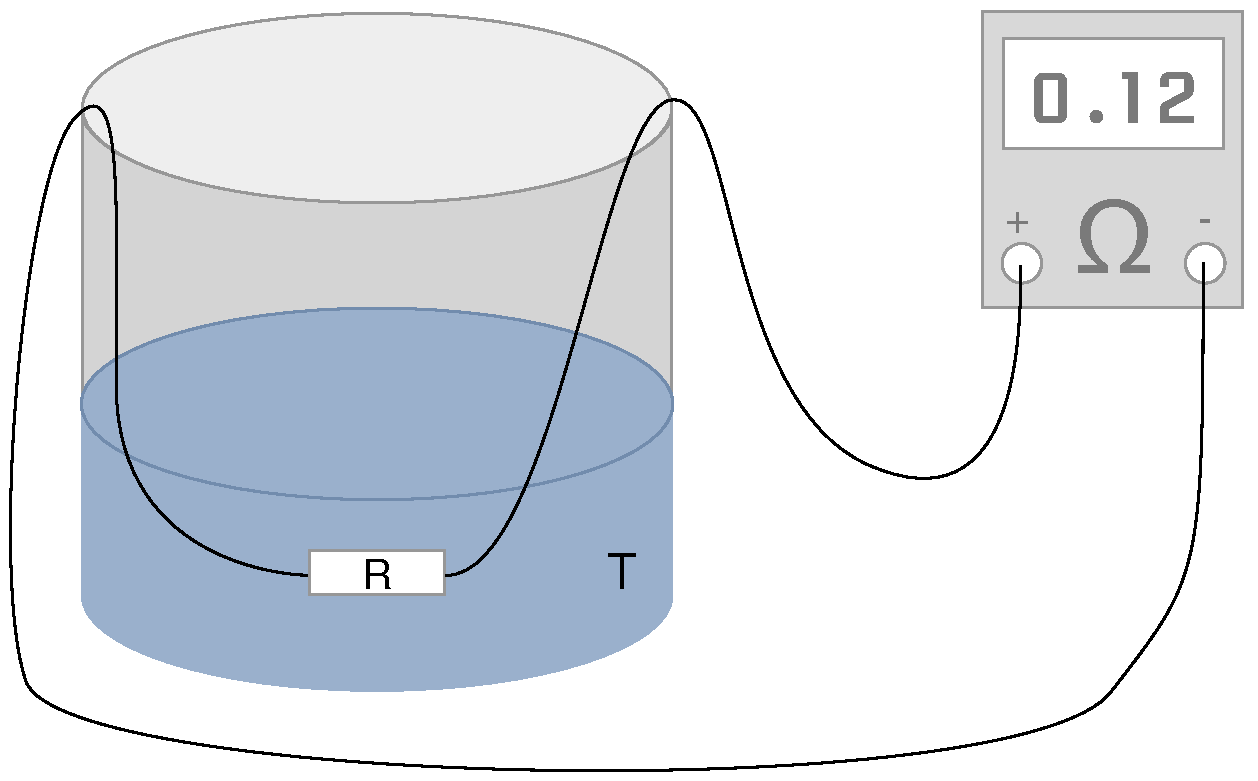
\includegraphics[width=\textwidth]{Bequer.pdf}
\caption{Desenho esquemático do experimento -- dentro de um béquer é colocada água com temperatura variando de $18ºC$ à $78ºC$ e mede-se a resistência elétrica correspondente do termoresistor.}
\label{fig:pt100-esquematico}
\end{figure}

\noindent
onde $R$ é um termoresistor Pt100, $T$ é a temperatura da água dentro do copo de Béquer, e o instrumento $\Omega$ é um ohmímetro.

As medidas foram feitas de forma aleatória e com 2 repetições por célula. Após a extração dos resultados, fez-se o ajuste de curvas e obteve-se a função de transferência experimental do termoresistor.

Com o copo de Béquer preenchido com água até a metade para que o processo de aquecimento não levasse muito tempo e nem que fosse necessário aguardar o aquecimento de um grande volume de água nem resfriar o mesmo. Uma vez que a temperatura da agua estivesse ajustada na temperatura desejada, o valor de resistência elétrica correspondente mostrado no multímetro foi anotado.

Para fazer o ajuste de temperatura da água até a temperatura de interesse foram utilizadas 2 práticas: o uso de um aquecedor elétrico para elevar a temperatura e adição de água gelada para abaixar a temperatura. Isto é, caso a temperatura de interesse estivesse acima da temperatura atual da água, um aquecedor elétrico foi utilizado para elevar a temperatura e comparar utilizando um termômetro comercial de referência e caso a temperatura de interesse estivesse abaixo da temperatura atual da água, uma pequena porção de água gelada foi adicionada ao copo até que a temperatura de desejo fosse obtida.

O termômetro comercial utilizado não possuía identificação com nome do fabricante mas informa que tem resolução de 0.1ºC dentro do intervalo de interesse com incerteza de 1ºC. Acredita-se (este fator não foi testado) que o termômetro faz uso de uma média móvel com janela entre 20 e 30 segundos devido ao tempo de resposta perceptível do termômetro durante a execução do experimento. Devido a isto, aguardava-se para que o valor mostrado no \textit{display} da referência estivesse, por, pelo menos, 10 segundos num valor estável.

Enquanto o aquecedor estava ligado ou logo após a adição de água gelada, com uma colher de plástico, a água era agitada para que a temperatura fosse homogeneizada por todo volume. Também foi tomado o devido cuidado para que o nem sensor nem o termômetro de referência ficassem muito próximos do aquecedor que poderia causar danos à eles ou provocar erros sistemáticos de medida devido ao super aquecimento interno nos componentes que não pudessem ser facilmente dissipados na duração do experimento.

Como \textit{ohmímetro} foi utilizado um multímetro digital da Minipa, modelo ET-2082b, que possui as especificações de precisão conforme é apresentada na Tabela \ref{tab:precisao-multimetro}. 

\begin{table}[H]
\centering
\caption{Especificações de Precisão do multímetro digital Minipa ET-2082b - Escala de resistência elétrica}
\label{tab:precisao-multimetro}
\begin{tabular}{|c|c|c|}
\hline
\textbf{Faixa} & \textbf{Precisão}                 & \textbf{Resolução} \\ \hline
200 $\Omega$           & $\pm$ (0.8\%+5D)                  & 0.1 $\Omega$                 \\ \hline
2 k$\Omega$             & \multirow{4}{*}{$\pm$ (0.8\%+3D)} & 1 $\Omega$                   \\ \cline{1-1} \cline{3-3} 
20 k$\Omega$            &                                   & 10 $\Omega$                  \\ \cline{1-1} \cline{3-3} 
200 k$\Omega$           &                                   & 100 $\Omega$                 \\ \cline{1-1} \cline{3-3} 
2 M$\Omega$             &                                   & 1 k$\Omega$                 \\ \hline
20 M$\Omega$            & $\pm$ (1.0\%+15D)                 & 10 k$\Omega$                \\ \hline
2000 M$\Omega$          & $\pm$ {[}5\%(Leit.-10D)+20D{]}    & 1 M$\Omega$                 \\ \hline
\end{tabular}
\end{table}

\todo{discussão sobre os amplificadores, como ele pede no roteiro}

\todo{resto do experimento do pt100}

\section{Sensor de temperatura baseado em NTC}
\label{ch:ntc}
\subsection{Calibração do sensor NTC}
O NTC (\textit{Negative Temperature Coefficient}) é um termoresistor, não-linear cujo coeficiente de temperatura é negativo e, portanto, sua resistência elétrica decai à medida que a temperatura se eleva.

Analogamente ao sensor de temperatura baseado em Pt100 (Página \pageref{ch:pt100}), para que seja possível a construção de um termômetro utilizando um sensor do tipo NTC, é necessário que primeiramente seja levantada a função de transferência do componente para que seja possível utilizá-la na cadeia de medidas do termômetro.

A função de transferência teórica do NTC é dada pela Equação \ref{eq:ntc} \cite{livro-texto}.

\begin{equation}
	\large
	R(T) \approxeq R_0 e^{\beta\left(\frac{1}{T} - \frac{1}{T_0}\right)}
	\label{eq:ntc}
\end{equation}

\noindent
onde $R(T)$ é a resistência elétrica em $\Omega$ do NTC para uma dada temperatura $T$ em $K$, $\beta$ é uma constante dependente do material e características de construção do NTC, $R_0$ é a resistência de referência em $\Omega$ e $T_0$ é a temperatura de referência do termoresistor em $K$.

Para estimar a função de transferência experimental do NTC, projetou-se um experimento onde foram feitas 2 medidas de forma aleatória para temperaturas de $18ºC$ até $78ºC$, graduadas em $2ºC$ cada. Na Figura \ref{fig:ntc-esquematico} está apresentado um desenho simplificado da configuração utilizada no experimento.

\begin{figure}[H]
\center
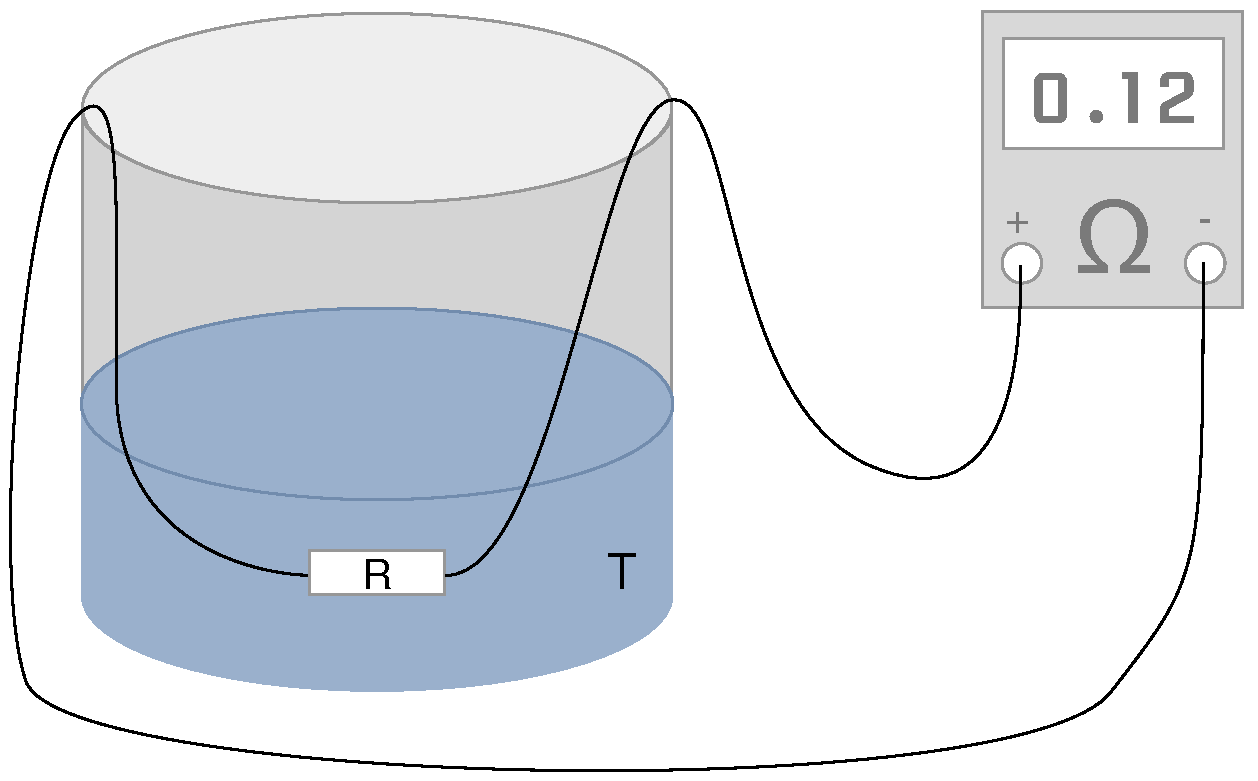
\includegraphics[width=\textwidth]{Bequer.pdf}
\caption{Desenho esquemático do experimento -- dentro de um béquer é colocada água com temperatura variando de $18ºC$ à $78ºC$ e mede-se a resistência elétrica correspondente do NTC.}
\label{fig:ntc-esquematico}
\end{figure}

\noindent
onde $R$ é um termoresistor NTC, $T$ é a temperatura da água dentro do copo de Béquer em $K$, e o instrumento $\Omega$ é um ohmímetro.

As medidas foram feitas de forma aleatória e com 2 repetições por célula. Após a extração dos resultados, fez-se o ajuste de curvas e obteve-se a função de transferência experimental do termoresistor.

A cadeia de medidas deste experimento é dada pela Figura \ref{fig:ntc-cadeia-medidas}:

\begin{figure}[H]
\center
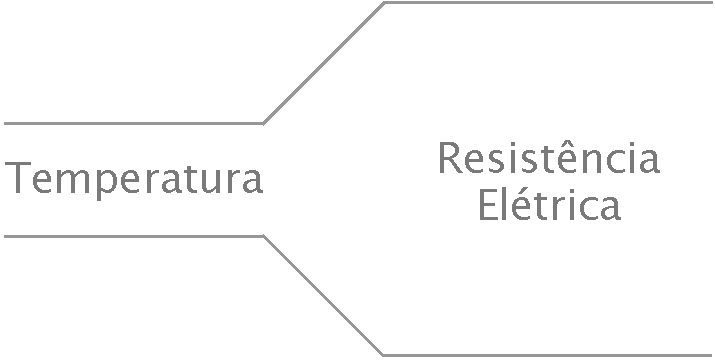
\includegraphics[width=0.7\textwidth]{CadeiaMedidas.pdf}
\caption{Cadeia de medidas para o sensor NTC}
\label{fig:ntc-cadeia-medidas}
\end{figure}

\noindent
onde a entrada é dada em temperatura (ºC) e a saída é dada em resistência elétrica ($\Omega$).



\section{Ponte de Wheatstone}

A próxima etapa da cadeia de medição passa por uma ponte de Whatstone, conforme apresentada na Figura \ref{fig:wheatstone}.

\begin{figure}[H]
\center
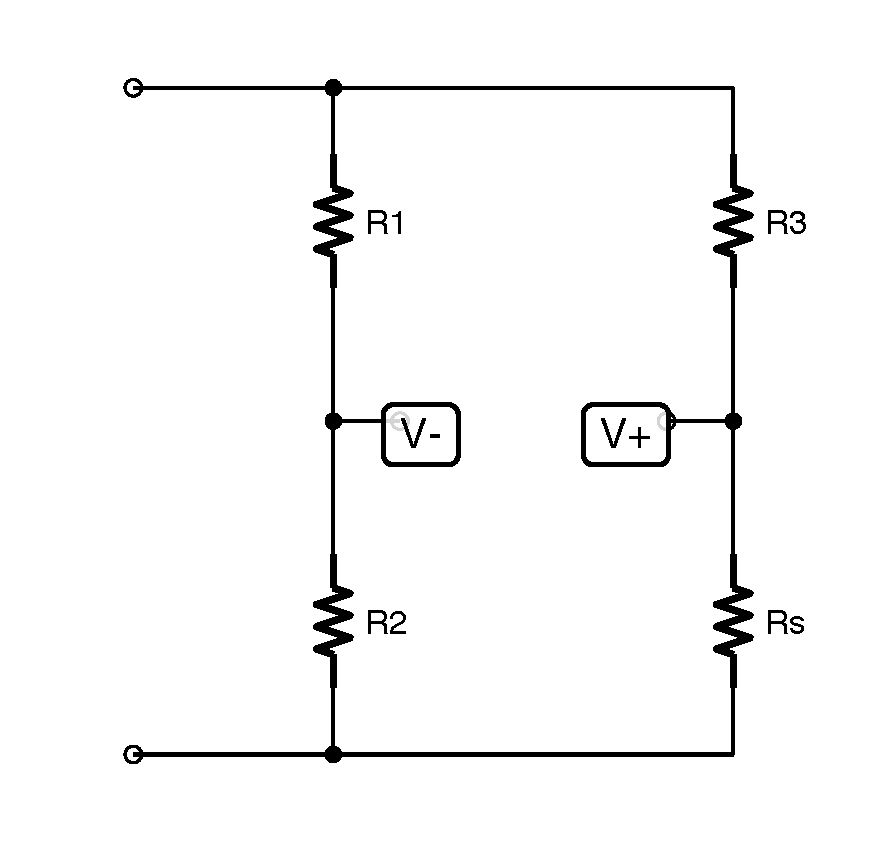
\includegraphics[width=0.7\textwidth]{Wheatstone.pdf}
\caption{Circuito elétrico da ponte de Wheatstone}
\label{fig:wheatstone}
\end{figure}

\noindent onde $R_1$, $R_2$ e $R_3$ são os valores de resistência elétrica calculadas para equilíbrio e sensibilidade de especificação da ponte, $R_s$ é a resistência elétrica do sensor (NTC e Pt100), $V-$ e $V+$ são as saídas em tensão elétrica.

A equação da tensão de saída da ponte é dada conforma a Equação \ref{eq:wheatstone}:

\begin{equation}
	V_o = \left({{R_2}\over{R_1 + R_2}} - {{R_s}\over{R_s + R_3}}\right)V_s
	\label{eq:wheatstone}
\end{equation}

\noindent onde $R_1$, $R_2$ e $R_3$ são os valores de resistência elétrica calculadas para equilíbrio e sensibilidade de especificação da ponte, $R_s$ é a resistência elétrica do sensor (NTC e Pt100), $V_0$ é a tensão elétrica diferencial de saída da ponte e $V_s$ é a tensão de alimentação da ponte.

Logo, é possível observar que para o caso em que a resistência elétrica do sensor é igual à resistência elétrica de $R_2$ a saída da ponte é de $0V$. Está situação é chamada de equilíbrio da ponte. Também é importante notar que qualquer incerteza no valor de tensão elétrica da fonte ($V_s$), incorre numa incerteza propagada no valor medido da saída da ponte ($V_o$), para tanto é importante que o valor de tensão elétrica de alimentação seja o mais estável e com menor incerteza possível para obter o melhor resultado.

\subsection{Equilíbrio da ponte de Wheatstone para o Pt100}
Uma vez que o Pt100 já possui comportamento linear, pode-se utilizar seu valor de resistência caraterístico diretamente na ponte. Uma vez que o intervalo de temperatura testadas não incluía a temperatura de $0ºC$, escolheu-se uma outra temperatura intermediária para fazer o equilíbrio da ponte. A fim de obter uma excursão de sinal maior, optou-se por utilizar o ponto médio de resistência elétrica como o ponto de equilíbrio. Este ponto favorece a excursão do sinal pois para temperaturas acima da referência, a tensão de saída da ponte se torna positiva, para temperaturas abaixo, a tensão de saída da ponte se torna negativa.

Dessa forma, considerando o intervalo de medição de resistência elétrica realizado na Seção \ref{sec:resistencia-pt100}, onde o intervalo estipulado foi de 18ºC até 76ºC, a temperatura média entre estes dois extremos é 47ºC, contudo as medidas foram realizadas com resolução de 2ºC, escolheu-se aproximar este valor para a temperatura de 46ºC. Dessa forma, temperaturas entre 48ºC até 76ºC devem fornecer um valor positivo de tensão elétrica na saída da ponte e temperaturas entre 18ºC até 44ºC devem fornecer um valor negativo de tensão elétrica na saída da ponte.

As Equações \ref{eq:ponte-wheatstone-pt100-sensibilidade} e \ref{eq:ponte-wheatstone-pt100-erro} apresentam as definições da sensibilidade e do erro de linearidade da ponte de Wheatstone aplicadas ao Pt100:


\begin{eqnarray}
	S = V_s \alpha \frac{r}{(r+1)}	 \label{eq:ponte-wheatstone-pt100-sensibilidade} \\
	\text{Erro de Linearidade} = \left|\frac{\alpha \Delta T}{r+1}\right|			   \label{eq:ponte-wheatstone-pt100-erro}
\end{eqnarray}

\noindent onde $V_s$ é a tensão elétrica de alimentação da ponte, $r$ é a razão característica da ponte, $\alpha$ é a constante característica do Pt100 e $\Delta T$ é a variação máxima de temperatura medida pelo sensor.

A razão característica da ponte de Wheatstone é definida de acordo com a Equação \ref{eq:ponte-wheatstone-pt100-razao}:

\begin{equation*}
	R_2 = R_3 = R = r R_0 \therefore
\end{equation*}
\begin{equation}
	r = \frac{R}{R_0}
	\label{eq:ponte-wheatstone-pt100-razao}
\end{equation}

\noindent onde $R_2$ e $R_3$ são resistores do braço inferior da ponte e $R_0$ é o valor de resistência elétrica de equilíbrio da ponte (valor de resistência em que a saída é zero).

\todo{falar sobre o erro de linearidade e senbilidade de projeto}

Na Tabela \ref{tab:pt100-ponte-resistores} estão apresentados os valores de resistências elétricas utilizadas na ponte de Wheatstone:

\begin{table}[H]
\centering
\caption{Valores de resistência elétrica da ponte de Wheatstone para sensor do tipo Pt100}
\label{tab:pt100-ponte-resistores}
\begin{tabular}{|c|c|c|}
\hline
	\textbf{Resistor} 	& \textbf{Valor nominal ($\Omega$)} 	& \textbf{Tolerância ($\Omega$)} 	\\ \hline
	$R_1$				& 100									& 10\%								\\ \hline
	$R_2$				& 100									& 10\%								\\ \hline
	$R_3$				& 100									& 10\%								\\ \hline
\end{tabular}
\end{table}
\todo{nao anotamos esses valores, precisamos recalcular ou descobrir eles}

Para alimentação da fonte, foi utilizada uma fonte \todo{fonte do lab} ajustada para tensão elétrica de $2V$ que foi medida utilizando um multímetro \todo{do rodrigo} com uma incerteza de \todo{qual?}. De acordo com os dados fornecidos no manual pelo fabricante da fonte, o \textit{ripple} de tensão da tensão elétrica de saída é insignificante no experimento e pode ser desprezada.

Para a aquisição dos dados foi utilizado uma placa de aquisição de dados comercial da National Instruments, modelo NI USB-6009, cujo conversor analógico-digital possui 14 bits\cite{daq-specifications}. Numa etapa anterior à amostragem, o sinal passou por um filtro passa-baixas de Butterworth de quarta ordem com frequência de corte de 100 Hz implementado na topologia de filtros ativos de Sallen-Key. No LabVIEW, foi configurado os limites de amostragem na margem de $\pm 1V$, logo o intervalo total de 14 bits corresponde ao limites de $-1V$ até $+1V$, uma excursão de $2V$ que resulta numa resolução de $0.12\text{ mV/bit}$.

\subsection{Linearização do NTC}
\label{sec:ntc-linearizacao}

Conforme indicado na Equação \ref{eq:ntc}, o NTC possui comportamento não-linear e, para realizar processamento utilizando eletrônica analógica no sinal, e se linearizado, o trabalho com este sinal se torna muito mais simples e direto. Para tanto, é possível utilizar o método de linearização do ponto médio que consiste em adicionar um resistor em paralelo com o sensor calculado a partir de três pontos da curva do sensor. Na Figura \ref{fig:ntc-linear} está apresentado o esquemático elétrico do método de linearização proposto.

\begin{figure}[H]
\center
[circuito]
\caption{Circuito elétrico da ponte de Wheatstone}
\label{fig:ntc-linear}
\end{figure}
\todo{circuito}

\noindent
onde $R_l$ é o valor numérico da resistência elétrica de linearização, $R_s$ é o sensor e $R$ é a resistência elétrica equivalente do sensor linearizado. É importante ressaltar que este método não oferece uma linearização perfeita, isto é, o método apenas tenta aproximar o comportamento linear da melhor forma possível nesta topologia.

A Equação \ref{eq:ntc-linear-paralelo} fornece a expressão matemática da associação de dois resistores em paralelo:

\begin{equation}
	\frac{1}{R_{eq}}=\frac{1}{R_s} + \frac{1}{R_L}
	\label{eq:ntc-linear-paralelo}
\end{equation}

\noindent
onde $R_{eq}$ é a resistência elétrica equivalente da associação e $R_T$ e $R_L$ são os valores das resistências elétricas do sensor e da resistência elétrica de linearização, respectivamente.

Isolando-se o termo $R_{eq}$ da Equação \ref{eq:ntc-linear-paralelo}, resulta a Equação \ref{eq:ntc-linear-paralelo-isolado}, que representa o valor de resistência elétrica do sensor linearizado.

\begin{equation}
	R_{\text{linear}} = \frac{R_L R_T}{R_L+R_T}
	\label{eq:ntc-linear-paralelo-isolado}
\end{equation}

É fácil observar que há uma relação inversa da resistência elétrica, o formato da curva da função $1/x$ é muito próximo de uma função do tipo $e^{-x}$, conforme é possível observar graficamente na Figura \ref{fig:ntc-linear-funcao-comparacao}:

\begin{figure}[H]
\center
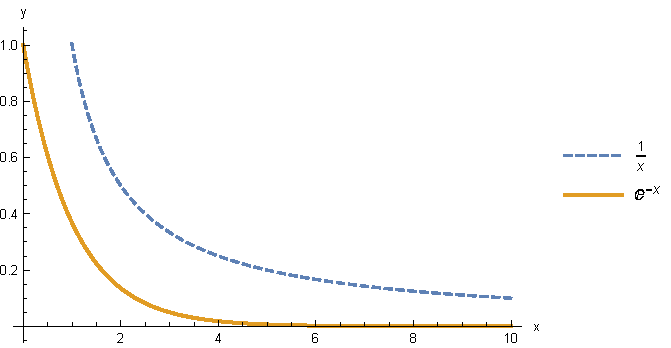
\includegraphics[width=\textwidth]{X1-vs-Exponencial.pdf}
\caption{Comparação entre a função $1/x$ e a função $e^{-x}$}
\label{fig:ntc-linear-funcao-comparacao}
\end{figure}

Desta forma, é possível aproximar o comportamento da ponte para que pareça linear, isto é, tenha um erro de linearidade baixo e, portanto, pode-se desprezar qualquer termo não linear na expressão da ponte.

Sabe-se que a expressão de saída da ponte de Wheatstone, é dada pela Equação \ref{eq:ponte-wheatstone}:

\begin{equation}
	V(T) = V_s \frac{(R_1 R(T)- R_1 R_3)}{(R_1+R(T)) (R_2+R_3)}
	\label{eq:ponte-wheatstone}
\end{equation}

\noindent onde $V(T)$ é a tensão elétrica de saída da ponte para uma temperatura $T$, $R_1$, $R_2$ e $R_3$ são resistores que definem as características da ponte, $R(T)$ é o elemento resistivo sensível a temperatura (NTC) e $V_s$ é a tensão elétrica de alimentação da ponte.

Considerando que $R_s$ seja a resistência elétrica do sensor linearizado conforme dada pela Equação \ref{eq:ntc-linear-paralelo-isolado}, pode-se substituir a Equação \ref{eq:ntc-linear-paralelo-isolado} na Equação \ref{eq:ponte-wheatstone} com a substituição de variáveis para obter a Equação \ref{eq:ponte-wheatstone-ntc} da ponte de Wheatstone linearizada.

\begin{equation}
	V(T) = \frac{V_s \left(\frac{R_1}{\frac{1}{R_L}+\frac{1}{R(T)}}-R_1 R_3\right)}{(R_2+R_3) \left(R_1+\frac{1}{\frac{1}{R_L}+\frac{1}{R(T)}}\right)}
	\label{eq:ponte-wheatstone-ntc}
\end{equation}

\noindent onde $V(T)$ é a tensão elétrica de saída da ponte para uma temperatura $T$, $R_1$, $R_2$ e $R_3$ são resistores que definem as características da ponte, $R(T)$ é o elemento resistivo sensível a temperatura (NTC), $R_L$ é o sensor em paralelo ao sensor de temperatura NTC e $V_s$ é a tensão elétrica de alimentação da ponte.

O processo apresentado é funcional e a saída tem um erro de linearidade bem baixo (é quase imperceptível a curvatura da curva de medida), mas há outro problema; a corrente que circula pelo NTC causará um erro de auto aquecimento do termoresistor, que, se não controlado, poderá causar sérios erros na medida de tensão elétrica em função da temperatura na saída da ponte. Para compensar este efeito, um resistor em série com o sensor será adicionado para que a corrente circulando pelo sensor seja limitada até um valor aceitável, que é definido pelo erro de auto aquecimento máximo tolerável pelo projeto. Na Equação \ref{eq:ntc-linear-sensor-serie}, está apresentada a equação equivalente do sensor e seu resistor série:

\begin{equation}
	R_{\text{limitado}}(T) = R_s + R(T)
	\label{eq:ntc-linear-sensor-serie}
\end{equation}

\noindent onde $R_{\text{limitado}}(T)$ é a resistência elétrica equivalente com a corrente limitada, $R_s$ é a resistência elétrica série que faz o limite de corrente e $R(T)$ é a resistência elétrica do sensor. Substituindo a Equação \ref{eq:ntc-linear-sensor-serie} na Equação \ref{eq:ponte-wheatstone-ntc}, obtém-se a Equação \ref{eq:ponte-wheatstone-ntc-limitado} que representa a mesma ponte de Equação \ref{eq:ponte-wheatstone-ntc}, mas dessa vez com o resistor de limite de corrente:

\begin{equation}
	V(T) = \frac{V_s \left(\frac{R_1}{\frac{1}{R_L}+\frac{1}{R_s+R_T}}-R_1 R_3\right)}{(R_2+R_3) \left(R_1+\frac{1}{\frac{1}{R_L}+\frac{1}{R_s+R_T}}\right)}
	\label{eq:ponte-wheatstone-ntc-limitado}
\end{equation}

Da equação \ref{eq:ponte-wheatstone-ntc-limitado}, é possível extrair as equações correspondentes à sensibilidade (Equação \ref{eq:ponte-wheatstone-ntc-sensibilidade}) e ao erro de linearidade da ponte linearizada  (Equação \ref{eq:ponte-wheatstone-ntc-erro}).

\begin{eqnarray}
	S 							= ...			\\ \label{eq:ponte-wheatstone-ntc-sensibilidade}
	\text{Erro de Linearidade} = ...			 	   \label{eq:ponte-wheatstone-ntc-erro}
\end{eqnarray}

\todo{equações anteriores}

Por definição de projeto, adotou-se um erro de linearidade máximo de $20\%$ e sensibilidade de $0.2 V$. 

\subsection{Equilíbrio da ponte de Wheatstone para o NTC}

\todo{apresentar os calculos dos resistores}

Na Figura \ref{fig:ntc-linear-esperado} está apresentado a curva esperada da saída da ponte para o NTC linearizado:

\begin{figure}[H]
\center
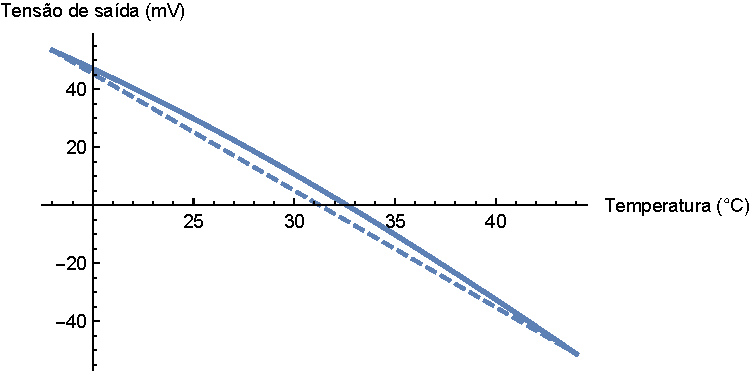
\includegraphics[width=\textwidth]{NTC-Linear-Esperado.pdf}
\caption{Curva de saída esperada da ponte para o NTC linearizado}
\label{fig:ntc-linear-esperado}
\end{figure}

Na Figura \ref{fig:ntc-linear-esperado} a linha contínua é o valor real da linearização (note que a curva não é perfeitamente linear) e a linha tracejada é a curva desprezando componentes não lineares da curva contínua. É fácil observar que o erro de linearidade nas extremidades tende à zero e no ponto médio é máximo. Isso mostra que a linearização proposta não é perfeita, e possui um erro de linearidade intrínseco atrelado, mas se comparado com o formato da curva bruta, sem linearização, o resultado obtido possui um erro de linearidade muito inferior, isto é, a forma linearizada é muito mais linear que a forma não linear.

\chapter{Resultados e Discussões}
\section{Sensor de temperatura baseado em Pt100}
Com base na metodologia apresentada na seção \ref{ch:pt100} da Metodologia Experimental, foram levantadas os valores da resistência elétrica para o sensor Pt100, na faixa especificada, com 2 amostras por temperatura. Os resultados são observados da Tabela \ref{tab:amostras-pt100}, que mostra também uma coluna com o valor médio para cada temperatura, com base nas duas medições. O multímetro foi utilizado na escala de resistência elétrica, para a faixa de 200 $\Omega$, e possui precisão e resolução conforme apresenta da Tabela \ref{tab:precisao-multimetro}.

\begin{table}[H]
\centering
\caption{Amostras de medidas de resistência elétrica do Pt100 - Temperatura 18ºC a 76ºC}
\label{tab:amostras-pt100}
\begin{tabular}{|c|c|c|c|}
\hline
\textbf{Temp. ($ºC$)} & \textbf{Medida 1 ($\Omega$)} & \textbf{Medida 2 ($\Omega$)} & \textbf{Média ($\Omega$)} \\ \hline
18                  & 106,8                 & 107,0                 & 106,9          \\ \hline
20                  & 108,4                 & 108,1                 & 108,3          \\ \hline
22                  & 109,0                 & 108,9                 & 109,0          \\ \hline
24                  & 109,4                 & 109,6                 & 109,5          \\ \hline
26                  & 110,2                 & 110,4                 & 110,3          \\ \hline
28                  & 111,0                 & 111,1                 & 111,1          \\ \hline
30                  & 111,9                 & 111,9                 & 111,9          \\ \hline
32                  & 112,7                 & 112,5                 & 112,6          \\ \hline
34                  & 113,3                 & 113,5                 & 113,4          \\ \hline
36                  & 114,1                 & 114,2                 & 114,2          \\ \hline
38                  & 115,0                 & 114,9                 & 115,0          \\ \hline
40                  & 115,7                 & 115,8                 & 115,8          \\ \hline
42                  & 116,6                 & 116,4                 & 116,5          \\ \hline
44                  & 117,3                 & 117,4                 & 117,4          \\ \hline
46                  & 117,9                 & 118,1                 & 118,0          \\ \hline
48                  & 118,8                 & 118,8                 & 118,8          \\ \hline
50                  & 119,5                 & 119,7                 & 119,6          \\ \hline
52                  & 120,8                 & 120,6                 & 120,7          \\ \hline
54                  & 121,1                 & 121,0                 & 121,1          \\ \hline
56                  & 121,7                 & 121,7                 & 121,7          \\ \hline
58                  & 122,7                 & 123,0                 & 122,9          \\ \hline
60                  & 123,4                 & 123,3                 & 123,4          \\ \hline
62                  & 124,4                 & 124,1                 & 124,3          \\ \hline
64                  & 124,8                 & 124,8                 & 124,8          \\ \hline
66                  & 125,4                 & 125,5                 & 125,5          \\ \hline
68                  & 126,3                 & 126,3                 & 126,3          \\ \hline
70                  & 127,0                 & 126,8                 & 126,9          \\ \hline
72                  & 128,0                 & 127,9                 & 128,0          \\ \hline
74                  & 128,6                 & 128,5                 & 128,6          \\ \hline
76                  & 129,1                 & 129,3                 & 129,2          \\ \hline
\end{tabular}
\end{table}

A Figura \ref{fig:pt100-amostras} \todo{verificar se fica esse ou faz outro gráfico no Mathematica} mostra os pontos de temperatura verificados, bem como a curva ajustada para os valores obtidos.

\begin{figure}[H]
\center
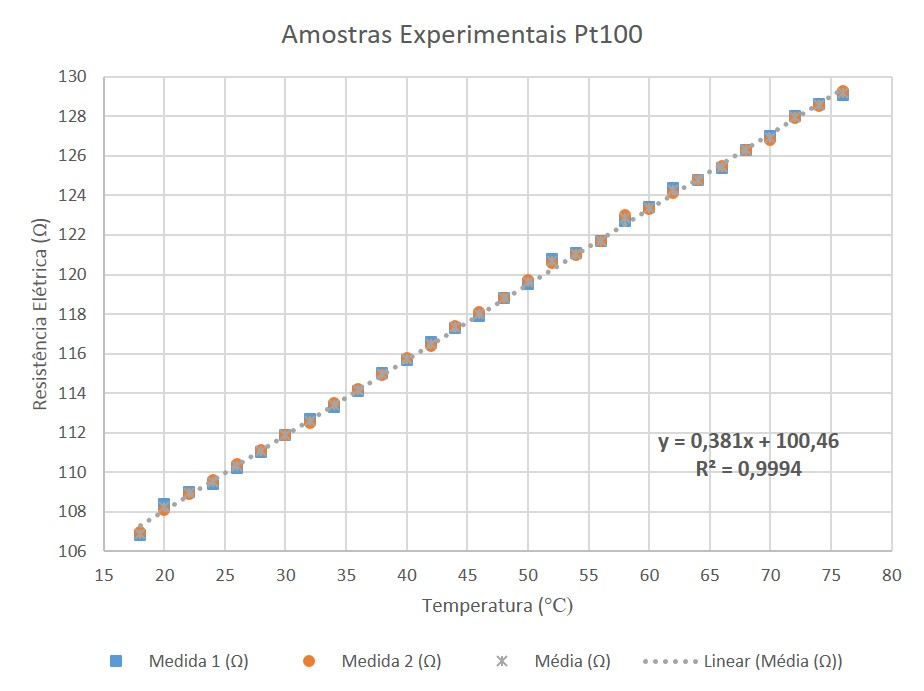
\includegraphics[width=0.7\textwidth]{pt100_puro.jpg}
\caption{Gráfico das amostras experimentais apresentando a variação da resistência elétrica em função da variação da temperatura da água.}
\label{fig:pt100-amostras}
\end{figure}

A regressão linear, com base nos valores da média das amostras obtidas, apresentou como função de transferência experimental os seguintes resultados:

\begin{equation}
	R(T) = 0.381*T + 100.46
	\label{eq:pt100-reg}
\end{equation}
\begin{equation}
	R^2=0.9994
	\label{eq:pt100-reg-r2}
\end{equation}

\noindent
onde $R(T)$ é a resistência elétrica, em $\Omega$, do sensor Pt100, e $T$ é a temperatura, em $ºC$, percebida pelo sensor.

A Equação \ref{eq:pt100-reg-r2} apresenta o valor do coeficiente de linearidade, significando que 99,94\% da variável dependente consegue ser explicada pelos regressores presentes no modelo.

Com base na Equação \ref{eq:pt100-alpha} pode-se facilmente encontrar o valor do coeficiente de temperatura $\alpha$. Também é possível notar, igualando as Equações \ref{eq:pt100} e \ref{eq:pt100-reg}, que:

\begin{eqnarray}
	R_0 &=& 100.46 [\Omega]\\
	\alpha R_0 &=& 0.381 [\frac{\Omega}{ºC}] \label{eq:pt100-alpha-valor}
\end{eqnarray}

De onde se pode extrair o valor de $\alpha$:
\begin{eqnarray}
	\alpha &=& \frac{0.381}{R_0} \\
	       &=& 0.00379 [\frac{\Omega}{\Omega ºC}]
\end{eqnarray}

O valor de $\alpha$ encontrado experimentalmente é compatível com o valor tabelado pela Norma \textit{IEC 751}, que é de 0.00385 $\frac{\Omega}{\Omega ºC}$ para \textit{RTDs} de Platina, que é o caso do Pt100.

Nota-se ainda que a Equação \ref{eq:pt100-alpha-valor} apresenta o valor da sensibilidade $S_{Pt100}$ do sensor.


\section{Sensor de temperatura baseado em NTC}

Na Tabela \ref{tab:amostras-ntc}, estão apresentados os valores de resistência elétrica do NTC que foram obtidas em função da temperatura do termoresistor.


\begin{table}[H]
\centering
\caption{Amostras de medidas de resistência elétrica do NTC - Temperatura 18ºC a 74ºC}
\label{tab:amostras-ntc}
\begin{tabular}{|c|c|c|c|}
\hline
\textbf{Temp. ($ºC$)} & \textbf{Medida 1 ($\Omega$)} & \textbf{Medida 2 ($\Omega$)} & \textbf{Escala} \\ \hline
 16 & 3340 & 3330 & \textit{Auto-scale} \\ \hline
 18 & 3000 & 3000 & \textit{Auto-scale} \\ \hline
 20 & 2810 & 2770 & \textit{Auto-scale} \\ \hline
 22 & 2590 & 2530 & \textit{Auto-scale} \\ \hline
 24 & 2380 & 2400 & \textit{Auto-scale} \\ \hline
 26 & 2180 & 2160 & \textit{Auto-scale} \\ \hline
 28 & 1990 & 1970 & \textit{Auto-scale} \\ \hline
 30 & 1790 & 1770 & \textit{Auto-scale} \\ \hline
 32 & 1650 & 1640 & \textit{Auto-scale} \\ \hline
 34 & 1540 & 1520 & \textit{Auto-scale} \\ \hline
 36 & 1360 & 1380 & \textit{Auto-scale} \\ \hline
 38 & 1310 & 1300 & \textit{Auto-scale} \\ \hline
 40 & 1210 & 1180 & \textit{Auto-scale} \\ \hline
 42 & 1110 & 1090 & \textit{Auto-scale} \\ \hline
 44 & 1020 & 990 & \textit{Auto-scale} \\ \hline
 46 & 950 & 930 & \textit{Auto-scale} \\ \hline
 48 & 860 & 880 & \textit{Auto-scale} \\ \hline
 50 & 810 & 790 & \textit{Auto-scale} \\ \hline
 52 & 740 & 740 & \textit{Auto-scale} \\ \hline
 54 & 690 & 680 & \textit{Auto-scale} \\ \hline
 56 & 630 & 630 & \textit{Auto-scale} \\ \hline
 58 & 580 & 580 & \textit{Auto-scale} \\ \hline
 60 & 560 & 550 & \textit{Auto-scale} \\ \hline
 62 & 520 & 510 & \textit{Auto-scale} \\ \hline
 64 & 470 & 480 & \textit{Auto-scale} \\ \hline
 66 & 460 & 440 & \textit{Auto-scale} \\ \hline
 68 & 420 & 420 & \textit{Auto-scale} \\ \hline
 70 & 380 & 380 & \textit{Auto-scale} \\ \hline
 72 & 360 & 360 & \textit{Auto-scale} \\ \hline
 74 & 340 & 330 & \textit{Auto-scale} \\ \hline
\end{tabular}
\end{table}


Na figura \ref{fig:ntc-medidas} está apresentado um gráfico de pontos onde cada ponto corresponde à uma medida realizada experimentalmente.

\begin{figure}[H]
\center
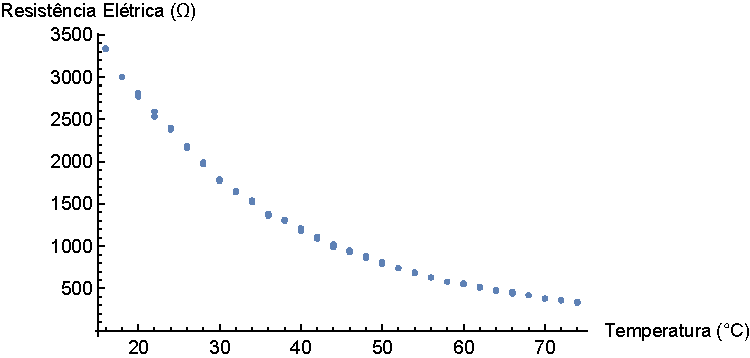
\includegraphics[width=\textwidth]{NTC-MeasurementsPlot.pdf}
\caption{Gráfico apresentando as medidas realizadas}
\label{fig:ntc-medidas}
\end{figure}

Com isto, pode-se fazer um ajuste de curvas não-linear utilizando a Equação \ref{eq:ntc} como formato de equação para o ajuste para obter a função de transferência experimental do termoresistor. Na Equação \ref{eq:ntc-experimental}, está dada a função de transferência resultante do ajuste:

\begin{equation} \large
	R(T) = 0.0043 e^{\frac{3920.77}{T+273}}
	\label{eq:ntc-experimental}
\end{equation}

\noindent onde $R(T)$ é a resistência elétrica em $\Omega$ do termoresistor e $T$ é a temperatura em $ºC$.

O ajuste foi realizado com um erro de conformidade $R^2$ dado pela Equação \ref{eq:ntc-experimental-erro}:

\begin{equation}
	R^2 = 0.9998
	\label{eq:ntc-experimental-erro}
\end{equation}

A título de comparação entre a função de transferência ajustada e os pontos medidos individualmente, a Figura \ref{fig:ntc-experimental-comparacao} apresenta a sobreposição entre o gráfico da Figura \ref{fig:ntc-medidas} e a curva da Equação \ref{eq:ntc-experimental}.

\begin{figure}[H]
\center
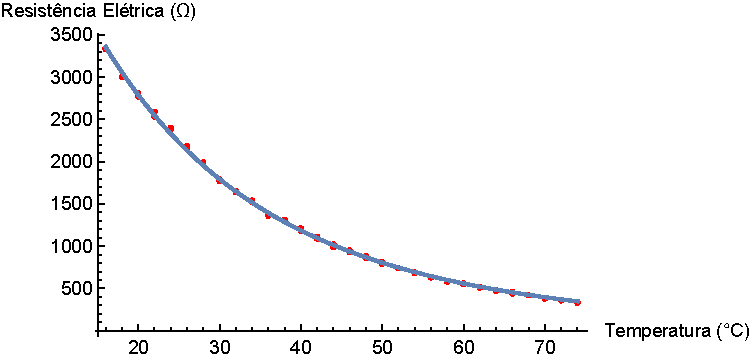
\includegraphics[width=\textwidth]{NTC-FitPlot.pdf}
\caption{Comparação entre as medidas individuais e a função de transferência ajustada}
\label{ntc-experimental-comparacao}
\end{figure}

Para realizar a linearização do NTC, foi escolhido o intervalo de 18ºC até 44ºC para linearizar através do método à 3 pontos equidistantes conforme explicado no capítulo de Metodologia Experimental, página \pageref{sec:ntc-linearizacao}.

Para tanto, foram feitas 3 medidas em 3 pontos, nos dois extremos (18 e 44 ºC) e no ponto médio (32 ºC). A Tabela \ref{tab:ntc-linearizado} apresenta os valores de tensão elétrica medida na saída da ponte com o sensor linearizado conectado.

\begin{table}[H]
\centering
\caption{Medidas de tensão elétrica na saída da ponte de Wheatstone para o sensor NTC linearizado. É importante lembrar que estas medidas foram feitas utilizando o dispositivo de aquisição de dados no LabVIEW.}
\label{tab:amostras-linearizado}
\begin{tabular}{|c|c|}
\hline
\textbf{Temp. ($ºC$)} & \textbf{Tensão elétrica (mV)} \\ \hline
 18 & 50.7  \\ \hline
 20 & 43.8  \\ \hline
 22 & 38.1  \\ \hline
 24 & 31.1  \\ \hline
 26 & 23.9  \\ \hline
 28 & 18.6  \\ \hline
 30 & 9.8   \\ \hline
 32 & 2.1   \\ \hline
 34 & -8.1  \\ \hline
 36 & -15.7 \\ \hline
 38 & -23.7 \\ \hline
 40 & -36.1 \\ \hline
 42 & -42.9 \\ \hline
 44 & -53.9 \\ \hline
\end{tabular}
\end{table}

A Figura \ref{fig:ntc-linear-obtido} apresenta a comparação entre uma linearização perfeita, a curva linearizada esperada e os valores obtidos experimentalmente.

\begin{figure}[H]
\center
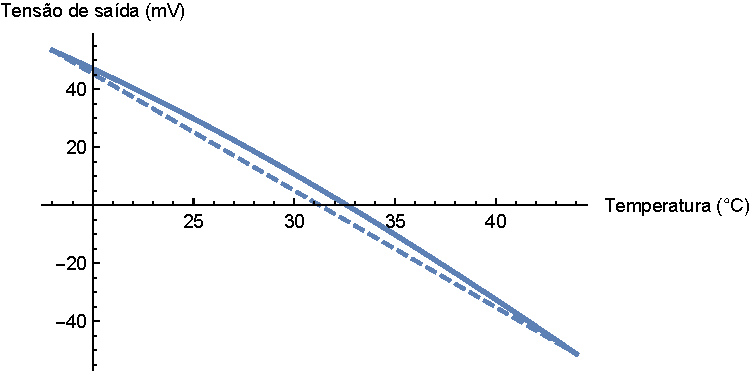
\includegraphics[width=\textwidth]{NTC-Linear-Obtido.pdf}
\caption{Comparação entre as medidas individuais e a função de transferência ajustada}
\label{ntc-experimental-comparacao}
\end{figure}

\noindent onde a linha contínua representa a curva esperada da linearização, a linha tracejada indica uma reta ligando os extremos da região de interesse e os pontos indicam as medidas realizadas experimentalmente.

A reta que melhor ajusta os dados experimentais da Tabela \ref{tab:amostras-linearizado} e da Figura \ref{ntc-experimental-comparacao}, é dada pela função da transferência na Equação \ref{eq:ntc-linearizado}:


\begin{equation}
	V(T) = 125 - 4.03 T
	\label{eq:ntc-linearizado}
\end{equation}

\noindent onde $V(T)$ é a tensão elétrica (em mV) de saída da ponte em função da temperatura $T$ em ºC.

Com a função de transferência linearizada do NTC na ponte de Wheatstone e utilizando o programa do LabVIEW desenvolvido, é possível extrair curvas da resposta temporal do sensor quando a temperatura a qual ele está submetido é variada bruscamente, isto é, quando é dado um choque térmico no sensor.

A Figura \ref{fig:ntc-choque-acima-tempo}, apresenta a resposta temporal do sensor quando submetido à uma diferença positiva de temperatura, isto é, quando ele é removido da água fria (18ºC) e colocado sobre um frasco com água quente (35ºC).

\begin{figure}[H]
\center
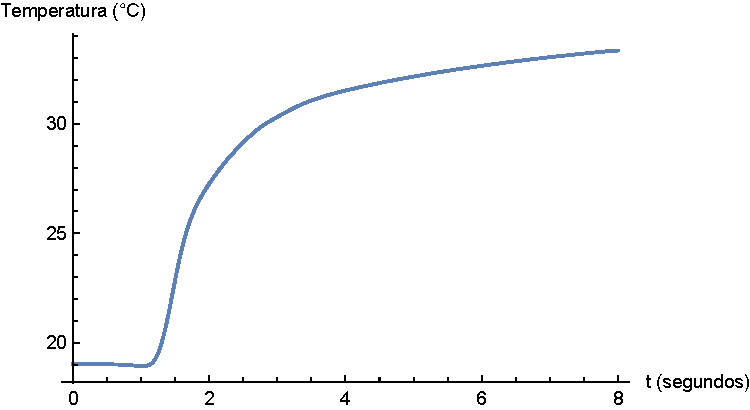
\includegraphics[width=\textwidth]{ThermalShock-Up-Time.pdf}
\caption{Curva de resposta do NTC no tempo ao dar um choque térmico de uma temperatura para outra superior (choque térmico de aquecimento)}
\label{fig:ntc-choque-acima-tempo}
\end{figure}

Na Figura \ref{fig:ntc-choque-acima-tempo} é importante observar que o sensor foi posto em choque térmico logo após o marco de 1 segundo, de acordo com o gráfico, é possível observar que 70\% da variação de temperatura do sensor tem sua resposta em 2 segundos (variação de 18 até 30ºC). Os 5ºC restantes tem uma inércia muito mais alta e precisam de mais de 10 segundos para que o valor estabilize no valor real de temperatura da água.

Também é possível realizar a transformada de Fourier do sinal da Figura \ref{fig:ntc-choque-acima-tempo} e obter a resposta em frequência do choque térmico do sensor.

\begin{figure}[H]
\center
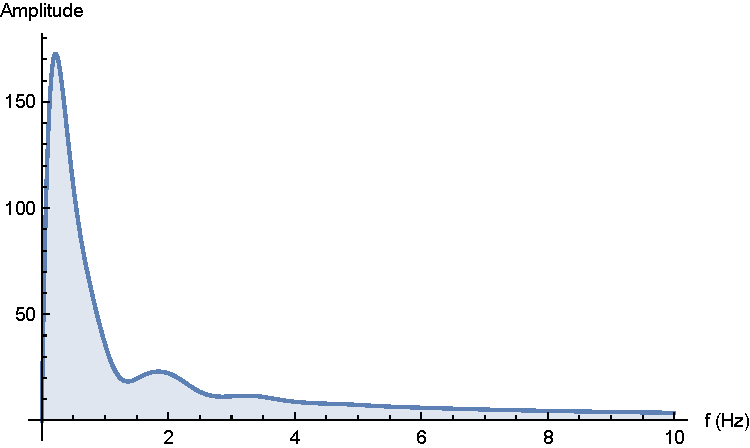
\includegraphics[width=\textwidth]{ThermalShock-Up-Frequency.pdf}
\caption{Transformada de Fourier da resposta do NTC no tempo ao dar um choque térmico de uma temperatura para outra superior (choque térmico de aquecimento). Foi feito uma interpolação utilizando uma \textit{Spline} de 10ª ordem para suavizar o espectro.}
\label{fig:ntc-choque-acima-frequencia}
\end{figure}

Na Transformada de Fourier do sinal, visto na Figura \ref{fig:ntc-choque-acima-frequencia} é possível comprovar as observações feitas sobre a resposta temporal. Isto é, a maior componente de frequência do sinal está em $0.5Hz$, que corresponde ao 2 segundos do tempo de estabilização de 70\% do valor de temperatura.

A curva para o processo inverso, um choque térmico de uma temperatura alta (35ºC) para outra baixa (18ºC) é apresentada na Figura \ref{fig:ntc-choque-abaixo-tempo}:

\begin{figure}[H]
\center
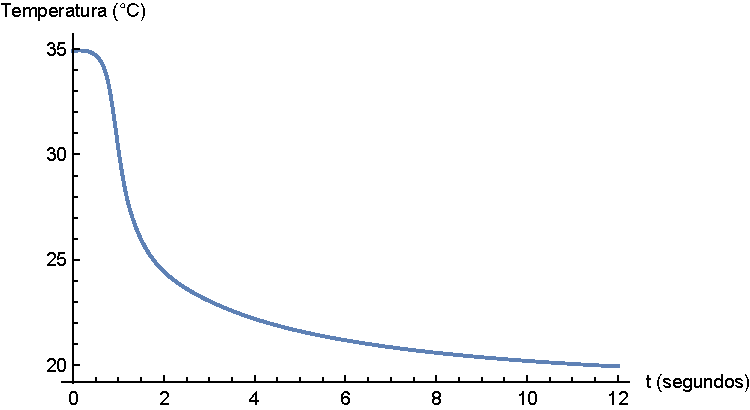
\includegraphics[width=\textwidth]{ThermalShock-Down-Time.pdf}
\caption{Curva de resposta do NTC no tempo ao dar um choque térmico de uma temperatura para outra inferior (choque térmico de resfriamento)}
\label{fig:ntc-choque-abaixo-tempo}
\end{figure}

Ao contrário do observado no choque térmico positivo, a variação de temperatura no primeiro segundo de após a troca de frasco é muito acentuada, a curva apresenta uma derivada altíssima, mas logo após o rebaixamento de 10ºC, a derivada começa a baixar rapidamente o valor até chegar ao marco de 12 segundos, onde o mesmo está entrando em regime permanente.

A análise em frequência da resposta transitória do sensor é apresentada na Figura \ref{fig:ntc-choque-abaixo-frequencia}.

\begin{figure}[H]
\center
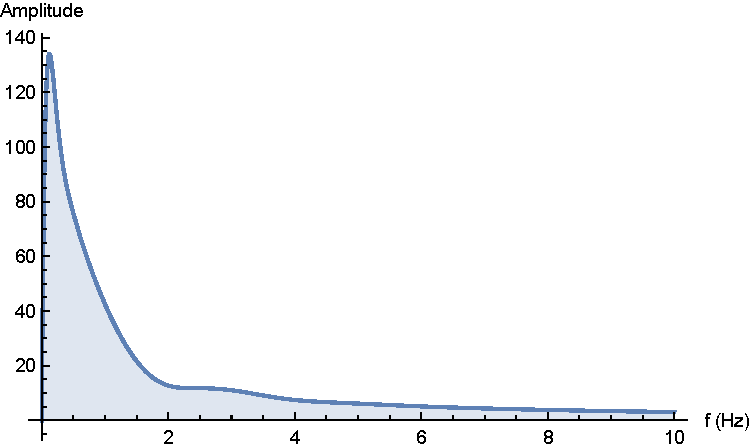
\includegraphics[width=\textwidth]{ThermalShock-Down-Frequency.pdf}
\caption{Transformada de Fourier da resposta do NTC no tempo ao dar um choque térmico de uma temperatura para outra inferior (choque térmico de resfriamento). Foi feito uma interpolação utilizando uma \textit{Spline} de 10ª ordem para suavizar o espectro.}
\label{fig:ntc-choque-abaixo-frequencia}
\end{figure}

Conforme afirmado na análise de resposta temporal, o primeiro segundo de variação apresenta uma variação altíssima, conforme pode ser observado na componente espectral de frequência em frequências baixas (abaixo de 1Hz) na Figura \ref{fig:ntc-choque-abaixo-frequencia}. Mas diferente do caso de aquecimento, no resfriamento a energia do espectro de potência do sinal se encontra mais disperso pelo espectro o que indica que sua resposta temporal é mais rápida comparada com o tempo de resposta do aquecimento.

Embora hajam diferenças nos tempos de acomodação das respostas apresentadas nas Figuras \ref{fig:ntc-choque-acima-tempo} e \ref{fig:ntc-choque-abaixo-tempo}, é visível que o sensor apresenta inércia térmica acima de 10s e seu uso seria impróprio para aplicações com frequências acima de $0.05Hz$, pois o sensor ainda não estaria em regime permanente e portanto incapaz de estimar a temperatura real.

\chapter{Conclusões}

\todo{lembrar as escalas dos multímetros, é importante mesmo. é a primeira coisa que ele enche o saco}

\newpage
\begin{thebibliography}{9}
\bibitem{mathematica-numerial-precision} \url{https://reference.wolfram.com/language/tutorial/NumericalPrecision.html}, acessado em 26 de abril de 2016
\bibitem{wikipedia-epsilon} \url{https://en.wikipedia.org/wiki/Machine_epsilon}, acessado em 26 de abril de 2016
\bibitem{livro-texto}  Balbinot, Alexandre; Brusamarello, Valner J., Instrumentação e Fundamentos de Medida - Vol.1 - 2ª Ed. Rio de Janeiro: LTC, 2014.

\bibitem{daq-specifications} NI USB-6009 -- DEVICE SPECIFICATIONS, \url{http://www.ni.com/pdf/manuals/375296a.pdf}, acessado em 3 de maio de 2016
\bibitem{daq-user-guide} NI USB-6009 -- USER GUIDE, \url{http://www.ni.com/pdf/manuals/371303n.pdf}, acessado em 3 de maio de 2016


%\bibitem{datasheet-lm7905} Datasheet oferecido pelo fabricante do regulador de tensão LM7905PI, disponível em \url{http://www.datasheetlib.com/datasheet/190159/kia7905pi_kec-korea-electronics-corporation.html}.

%\bibitem{datasheet-lm7805} Datasheet oferecido pelo fabricante do regulador de tensão LM7805CV, disponível em \url{http://www.datasheetlib.com/datasheet/221840/l7805cv_stmicroelectronics.html}.

%\bibitem{datasheet-lm741} Datasheet oferecido pelo fabricante do amplificador operacional LM741, disponível em \url{http://www.datasheetlib.com/datasheet/818655/lm741_ti-texas-instruments.html}.




%\bibitem{ref1} Sobrenome, A.B.; Sobrenome, C.D. Title of the cited article. Journal Title 2007, 6, 100-110. 
%\bibitem{ref2} Balbinot, A.; Brusamarello, V.J.. Title of the cited article. Journal Title 2007, 6, 100-110. 
%\bibitem{ref3} Author, A.; Author, B. Title of the chapter. In Book Title, 2nd ed.; Editor, A., Editor, B., Eds.; Publisher: Publisher Location, Country, 2007; Volume 3, pp. 154-196.
%\bibitem{ref4} Author, A.; Author, B. Book Title, 3rd ed.; Publisher: Publisher Location, Country, 2008; 
%pp. 154-196.

\end{thebibliography}

\iftoggle{attachments}{
	\chapter*{Anexos}
	\label{ch:attachments}
	\section{Mathematica}
	\includenotebook{../Resources/Mathematica/Experimento 1-1.nb.pdf}{Pêndulo}{pendulo}
	\includenotebooksingle{../Resources/Mathematica/Incerteza potenciometro.nb}{Incerteza do potenciômetro}{incerteza-potenciometro}
	\includenotebooksingle{../Resources/Mathematica/Incertezas-Filtro.nb}{Incerteza do filtro}{incerteza-filtro}

	\section{MATLAB}
	\label{att:script-matlab}
	\lstinputlisting[
		language=MATLAB,
		numbers=left,
		caption={Script MATLAB para análise de frequência}
	]{../Resources/MATLAB/primeiro.m}
}

\end{document}
